\documentclass[10pt,xcolor={svgnames}]{beamer}
%\usefonttheme[onlymath]{serif}
%%%%% Colors
\usetheme{Dresden}%\usetheme{Madrid}
\colorlet{beamer@blendedblue}{green!55!black}
%%%%%

%%%%% Other 
\addtobeamertemplate{navigation symbols}{}{%
    \usebeamerfont{footline}%
    \usebeamercolor[fg]{footline}%
    \hspace{1em}%
    \insertframenumber/\inserttotalframenumber
}
\usepackage{hyperref, url}

\definecolor{pine_green}{HTML}{007935}
\hypersetup{colorlinks,breaklinks,linkcolor=white,urlcolor=orange,citecolor=black}
\renewcommand\thefootnote{\textcolor{pine_green}{\arabic{footnote}}}
\setbeamercolor{alerted text}{fg=pine_green}

\renewcommand{\i}{\mathnormal{I}}

\usepackage{cancel}
\usepackage{ulem}
\usepackage{multirow}
\usepackage{mathtools}
\DeclarePairedDelimiter{\abs}{\lvert}{\rvert}
\renewcommand{\epsilon}{\varepsilon}
\setbeamertemplate{itemize subitem}{\textbullet}
\setbeamertemplate{itemize subsubitem}{$\circ$}

%https://tex.stackexchange.com/questions/289542/auto-resizing-parenthesis-in-math-formulas
% \usepackage{amsmath} for testing
\newcommand*\autoop{\left(}
\newcommand*\autocp{\right)}
\newcommand*\autoob{\left[}
\newcommand*\autocb{\right]}
\AtBeginDocument {%
   \mathcode`( 32768
   \mathcode`) 32768
   \mathcode`[ 32768
   \mathcode`] 32768
   \begingroup
       \lccode`\~`(
       \lowercase{%
   \endgroup
       \let~\autoop
   }\begingroup
       \lccode`\~`)
       \lowercase{%
   \endgroup
       \let~\autocp
   }\begingroup
       \lccode`\~`[
       \lowercase{%
   \endgroup
       \let~\autoob
   }\begingroup
       \lccode`\~`]
       \lowercase{%
   \endgroup
       \let~\autocb
   }}

\delimiterfactor 1001

\makeatletter
% for amsmath "compatibility" (not sophisticated)
% \usepackage{amsmath}
\AtBeginDocument {%
          \def\resetMathstrut@{%
           \setbox\z@\hbox{\the\textfont\symoperators\char40}%
           \ht\Mathstrutbox@\ht\z@ \dp\Mathstrutbox@\dp\z@}%
}%
\makeatother
%%%%%

%%%%% Greying out/invidible Slides
%\setbeamercovered{invisible}
%\setbeamercovered{%
%  again covered={\opaqueness<1->{15}}}
  
%%%%%







%%%%% Footnotes and captions
%\usepackage[utf8]{inputenc}
\usepackage{caption}
\usepackage{comment}
\setbeamerfont{footnote}{size=\tiny}
\setbeamerfont{caption}{size=\small}
%\setbeamerfont{normal text}{size=\small}
\setbeamerfont{itemize/enumerate body}{size=\small}
\setbeamerfont{itemize/enumerate subbody}{size=\footnotesize}
%%%%%



%Information to be included in the title page:
\title[Connor Wiegand]{Intro to Economic Analysis: Microeconomics}
\subtitle{EC 201 - Day 6 Slides}
\author[EC 201]{Connor Wiegand}
\institute[]{Department of Economics - University of Oregon}
\date{13 October 2021}


\begin{document}

\frame{\titlepage}

\begin{frame}{Logistics}
    \begin{itemize}
        \item Official homework 2 due this Saturday at 11:59pm, covering last week's material
        \item News assignments posted, first one due this Wednesday (October 13)
        \begin{itemize}
            \item This includes doing 1 news analysis of your choice on Cengage, \underline{and}
            \item Submitting a 1-1.5 page write up on Canvas
        \end{itemize}
        \item The outline must contain a brief summary of the article you read, as well as responses to the discussion questions that were at the end of your Cengage News Analysis    
        \end{itemize}
\end{frame}

\section*{Price Elasticity of Demand}

\begin{frame}{Recall}
    \begin{itemize}
        \item Formally, the price elasticity of demand (PED), denoted $e_{d}$, $E_{d}$, or, as I will use, $\epsilon_{D}$, is computed as
        $$\epsilon_{D}=\left|\frac{\%\Delta Q_{D}}{\%\Delta P}\right|$$
        where $\Delta$ is read ``change in"
        \item Using the midpoint method to calculate percentage change, this is given by 
        $$\epsilon_{D}=\left|\frac{\%\Delta Q_{D}}{\%\Delta P}\right|=\left|\frac{(Q_{2}-Q_{1})/[(Q_{1}+Q_{2})/2]}{(P_{2}-P_{1})/[(P_{1}+P_{2})/2]}\right|$$
    \end{itemize}
\end{frame}

\begin{frame}{Exercise 1}
    \begin{itemize}
        \item<1-> Recall the midpoint method:
        $$\Delta x=\frac{x_{2}-x_{1}}{(x_{1}+x_{2})/2}\cdot 100$$
        \item<2-> Suppose the price of a Juul is \$8. Your friend tells you that the price of Juul's has risen 25\% this year, and is for some reason using the midpoint method when they report the percentage
        \item<2-> Find the new price of a Juul
    \end{itemize}
\end{frame}

\begin{frame}{Solution 1}
    \begin{itemize}[<+->]
        \item So we have 
        \begin{align*}
            \Delta p=\frac{p_{2}-8}{(8+p_{2})/2}\cdot 100 &= 25\\
            \implies \frac{p_{2}-8}{(8+p_{2})}\cdot 2&=\frac{1}{4}\\
            \implies \frac{p_{2}-8}{p_{2}+8}&=\frac{1}{8}\\
            \visible<2->{\implies p_{2}-8 &=\frac{1}{8}p_{2}+1\\}
            \visible<3->{\implies \frac{7}{8}p_{2} &=9\\}
            \visible<4->{\implies p_{2} &=\frac{72}{7}\\}
        \end{align*}
        \item<5-> Therefore, $p_{2}\approx \$10.29$
    \end{itemize}
\end{frame}

\begin{frame}{PED Interpretation}
    \begin{itemize}[<+->]
        \item Suppose $\epsilon_{D}=2$ for burritos
        \item This says: ``if the price of burritos were to increase by 1\%, then the quantity demanded for burritos would fall by 2\%"
        \item In general, if good $x$ has PED $\epsilon_{D}$, then we would  say ``if the price of $x$ were to increase by 1\%, then the quantity demanded for $x$ would fall by $\epsilon_{D}$\%"
        \item If $\epsilon_{D}<1$, then $x$ is said to be \textit{inelastic}, and consumers are relatively insensitive to changes in the price of $x$
        \item If $\epsilon_{D}>1$, then $x$ is said to be \textit{elastic} and consumers are relatively sensitive to changes in the price of $x$
    \end{itemize}
\end{frame}


\begin{frame}{How PED Affects the Shape of a Demand Curve}
    \begin{itemize}[<+->]
        \item Generally speaking, a steeper demand curve reflects inelastic demand, while a flatter curve reflects elastic demand
        \item Consider rewriting the elasticity formula as 
        $$\epsilon_{D}=\left|\frac{\Delta Q_{D}}{\Delta P}\cdot \frac{(P_{1}+P_{2})/2}{(Q_{1}+Q_{2})/2}\right|$$
        \item Note that the absolute value of the slope of a [linear] demand curve is given by $|\Delta P/\Delta Q|$, so one of the terms above represents the reciprocal of the slope
        \item In other terms, a high value for the magnitude\footnote{In this context, another term for absolute value} of the slope will lead to a low $\epsilon_{D}$, \textit{all else equal}
        \begin{itemize}
            \item Inelastic demand $\implies$ low $\epsilon_{D}$ (close to 0) $\implies$ high $1/\epsilon_{D} \implies$ high $|\Delta P/\Delta Q| \implies $ steep slope
        \end{itemize}
    \end{itemize}
\end{frame}

\begin{frame}{Inelastic Demand}
    %\begin{figure}
        %\centering
        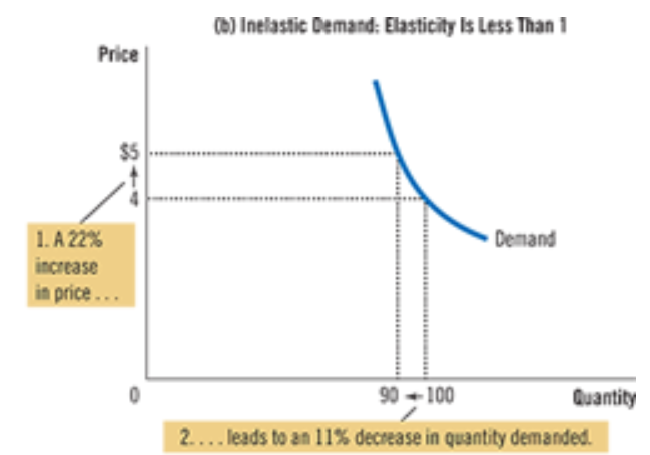
\includegraphics[width=8cm]{elastic demand from book-1.png} 
    %\end{figure}
\end{frame}

\begin{frame}{Elastic Demand}
    %\begin{figure}
        %\centering
        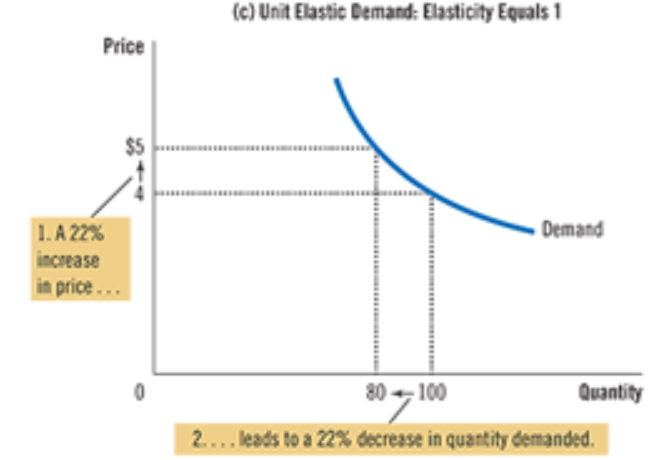
\includegraphics[width=8cm]{elastic demand from book-2.png} 
    %\end{figure}
\end{frame}

\begin{frame}{Unit-Elastic Demand}
    %\begin{figure}
        %\centering
        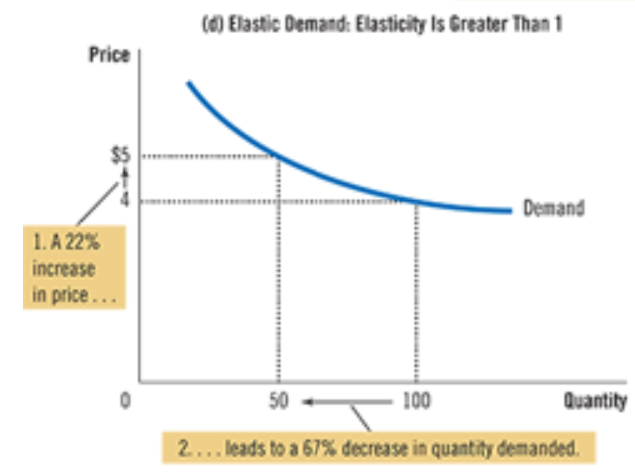
\includegraphics[width=8cm]{elastic demand from book-3.png} 
    %\end{figure}
\end{frame}

\begin{frame}{Mnemonic Device?}
\begin{table}[]
    \centering
    \begin{tabular}{c}
        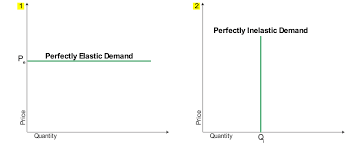
\includegraphics[width=8cm]{perfect elasticities.png}
    \end{tabular}
    \caption*{To remember which is which, just note that perfectly \underline{i}nelastic demand looks like an ``I", while perfectly \underline{e}lastic demand looks (kind of) like an ``E"}
\end{table}
\end{frame}

\begin{frame}{How PED Affects the Shape of a Demand Curve (cont.)}
    \begin{itemize}[<+->]
        \item Generally speaking, a steeper demand curve reflects inelastic demand, while a flatter curve reflects elastic demand
        \item In other terms, a high value for the magnitude\footnote{In this context, another term for absolute value} of the slope will lead to a low $\epsilon_{D}$, \textit{all else equal}
        \item This ``all else equal" statement is particularly important, because we are really trying to hold the midpoints equal
        \item Keep this in the back of your mind for later
    \end{itemize}
\end{frame}



%% New content
\begin{frame}{Portions of the Linear Demand Curve}
    \begin{itemize}[<+->]
        \item Remember rewriting the elasticity formula from earlier? When elasticity is allowed to be negative, 
        $$\epsilon_{D}=\frac{\Delta Q_{D}}{\Delta P}\cdot \frac{(P_{1}+P_{2})/2}{(Q_{1}+Q_{2})/2}$$
        \item What happens to that second term? 
        \item Consider the simple demand curve given by
        $$P=6-Q$$
        \url{https://www.desmos.com/calculator/2ihmjzo4hm}
        \item Calculate the elasticities between the following points:
        \begin{table}[H]
            \centering
            \begin{tabular}{c|c}
                $(6,0)$ and $(2,4)$ & $(2,4)$ and $(3,3)$ \\
                \hline
                $(3,3)$ and $(4,2)$ & $(4,2)$ and $(6,0)$ 
            \end{tabular}
        \end{table}
    \end{itemize}
\end{frame}

\begin{frame}{Portions of the Linear Demand Curve (cont.)}
    \begin{itemize}[<+->]
        \item Using $\epsilon_{D}=\left|\frac{\Delta Q_{D}}{\Delta P}\cdot \frac{(P_{1}+P_{2})/2}{(Q_{1}+Q_{2})/2}\right|$,
        \item $(0,6)\to(2,4)$:
            $$\frac{2-0}{|4-6|}\cdot \frac{(4+6)/2}{(2+0)/2}=1\cdot\frac{5}{1}=5$$
        \item $(2,4)\to(3,3)$:
            $$\frac{1}{|-1|}\cdot \frac{(3+4)/2}{(2+3)/2}=\frac{1}{|-1|}\cdot \frac{3.5}{2.5}=1\cdot1.4=1.4$$
        \item Notice that the first of these terms is always the inverse of the slope (in absolute value), so I always know between any two points on the curve, the first multiplier is 1
        \item I will now eyeball the midpoints for the second term. If you do not feel comfortable with this, go back through and verify these on your own
    \end{itemize}
\end{frame}

\begin{frame}{Portions of the Linear Demand Curve (cont.)}
    \begin{itemize}[<+->]
        \item<1-> Using $\epsilon_{D}=\left|\frac{\Delta Q_{D}}{\Delta P}\cdot \frac{(P_{1}+P_{2})/2}{(Q_{1}+Q_{2})/2}\right|$,
        \item<1-> $(0,6)\to(2,4)$:
            $$\frac{2-0}{|4-6|}\cdot \frac{(4+6)/2}{(2+0)/2}=1\cdot\frac{5}{1}=5$$
        \item<1-> $(2,4)\to(3,3)$:
            $$\frac{1}{|-1|}\cdot \frac{(3+4)/2}{(2+3)/2}=\frac{1}{|-1|}\cdot \frac{3.5}{2.5}=1\cdot1.4=1.4$$
        \item $(3,3)\to(4,2)$:
            $$\frac{1}{|-1|}\cdot \frac{2.5}{3.5}=0.71$$
        \item $(4,2)\to(6,0)$:
            $$\frac{2}{|-2|}\cdot \frac{1}{5}=0.2$$
    \end{itemize}
\end{frame}

\begin{frame}{What's happening?}
    \begin{itemize}[<+->]
        \item So, between 4 different sets of points, we have 4 different elasticities
        \item In fact, while the slope of the line remains constant, the elasticity varies along the curve, since the percentage change calculation is dependent on where you are on the curve
        \item In general, the portion of a linear demand curve that is above the midpoint is above the midpoint of the line\footnote{That is, the midpoint between the $x$ and $y$ intercepts} is elastic, while the below the midpoint is inelastic. At the midpoint, the PED is 1
    \end{itemize}
\end{frame}


\begin{frame}{A Subtle Distinction}
    \begin{itemize}[<+->]
        \item Before we dive into this next part, I will note that this is only for completeness, if you care
        \begin{itemize}
            \item If you do not, you are welcome to skip to the ``Takeaways" slide
        \end{itemize}
        \item Wait, if all linear demand curves have elastic and inelastic portions, then why do we say steeper demand curves are more inelastic?
    \end{itemize}
\end{frame}

\begin{frame}{A Subtle Distinction (cont.)}
    \begin{itemize}[<+->]
        \item Wait, if all linear demand curves have elastic and inelastic portions, then why do we say steeper demand curves are more inelastic?
        \item For recall the \textit{for all else equal} statement that I said to keep in mind earlier
        \item Fact: For two curves \underline{going through the same point}, the PED at (near) that point is smaller (more inelastic) for the steeper curve, and larger (more elastic) for the smaller curve (hence why we had to keep midpoints constant)
        \begin{itemize}
            \item Example: both (1) $P=24-6Q$ and (2) $P=4-\frac{1}{6}Q$ go through the point (3.49,3.49)
            \item If you calculate the PED for each of these curves such that $(3.49,3.49)$ is the midpoint of your two points\footnote{That is, you are calculating the PED between $(P_{1},Q_{1})$ and $(P_{2},Q_{2})$, and the midpoint is $(3.49,3.49)$}, you will get an elasticity of 
            \begin{align*}
                \epsilon_{D_{1}}=\frac{1}{6}\qquad\epsilon_{D_{2}}=6
            \end{align*}
            respectively
        \end{itemize}
    \end{itemize}
\end{frame}

\begin{frame}{A Subtle Distinction (cont.)}
    \begin{itemize}[<+->]
        \item Therefore, it is more ``shorthand" than technically correct to call steep curves inelastic and flat curves elastic
        \item However, since elasticity is related to slope, it is still common for economists to refer to steep demand curves as ``inelastic", and flat demand curves as ``elastic", even though elasticity varies along the curve
        \item To see why this is still okay, recall the diagram in the next slide\footnote{If this is not enough, hold tight for taxes, it will make more sense calling steep curves inelastic is okay.}
    \end{itemize}
\end{frame}

\begin{frame}{Graphical Understanding}
    \begin{figure}
        \centering
            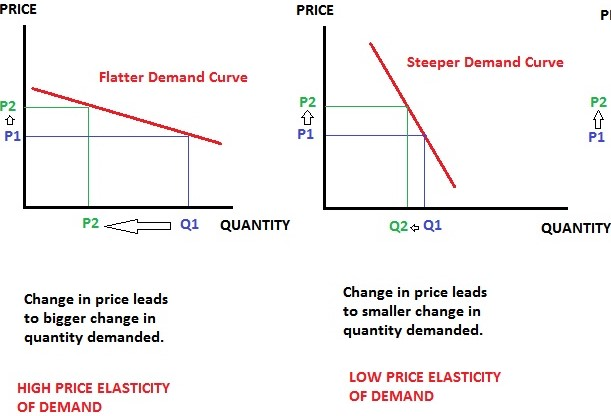
\includegraphics[width=7cm]{elastic v inelastic.jpg}
        \caption*{Note that the same level of price change leads to larger responses in flat curves than in steep curves. Therefore, when comparing more or less ``similar" curves, it makes sense to call one elastic and one inelastic, based on slope.}
    \end{figure}
\end{frame}


\begin{frame}{Takeaways}
    \begin{itemize}[<+->]
        \item If the above notes didn't make sense to you, I really just want you to 
        \begin{enumerate}
            \item Know how to calculate PED -- this is most important
            \item Know that PED varies along the demand curve, and know which portions are elastic/inelastic
            \item Know that when someone says "inelastic demand", they generally mean a relatively steep demand curve; when someone says ``elastic demand", they generally mean a relatively flat curve
            \begin{itemize}
                \item And don't worry too much about the numerical elasticity when someone says this 
            \end{itemize}
        \end{enumerate}
        \item Mankiw: ``The following rule of thumb is a useful guide: The flatter the demand curve passing through a given point, the greater the price elasticity of demand. The steeper the demand curve passing through a given point, the smaller the price elasticity of demand."
    \end{itemize}
\end{frame}

\section*{PED and Total Revenue}

\begin{frame}{Definition of Total Revenue}
    \begin{itemize}[<+->]
        \item Definition of Total Revenue (TR): $TR=P\cdot Q$
        \item Let's go back to a world without the supply curve; just suppose that I am picking a price to sell at, and then the consumers in the market show up to buy.
        \item My total revenue, $PQ$, is visualized in the following diagram:
        \begin{figure}
            \centering
            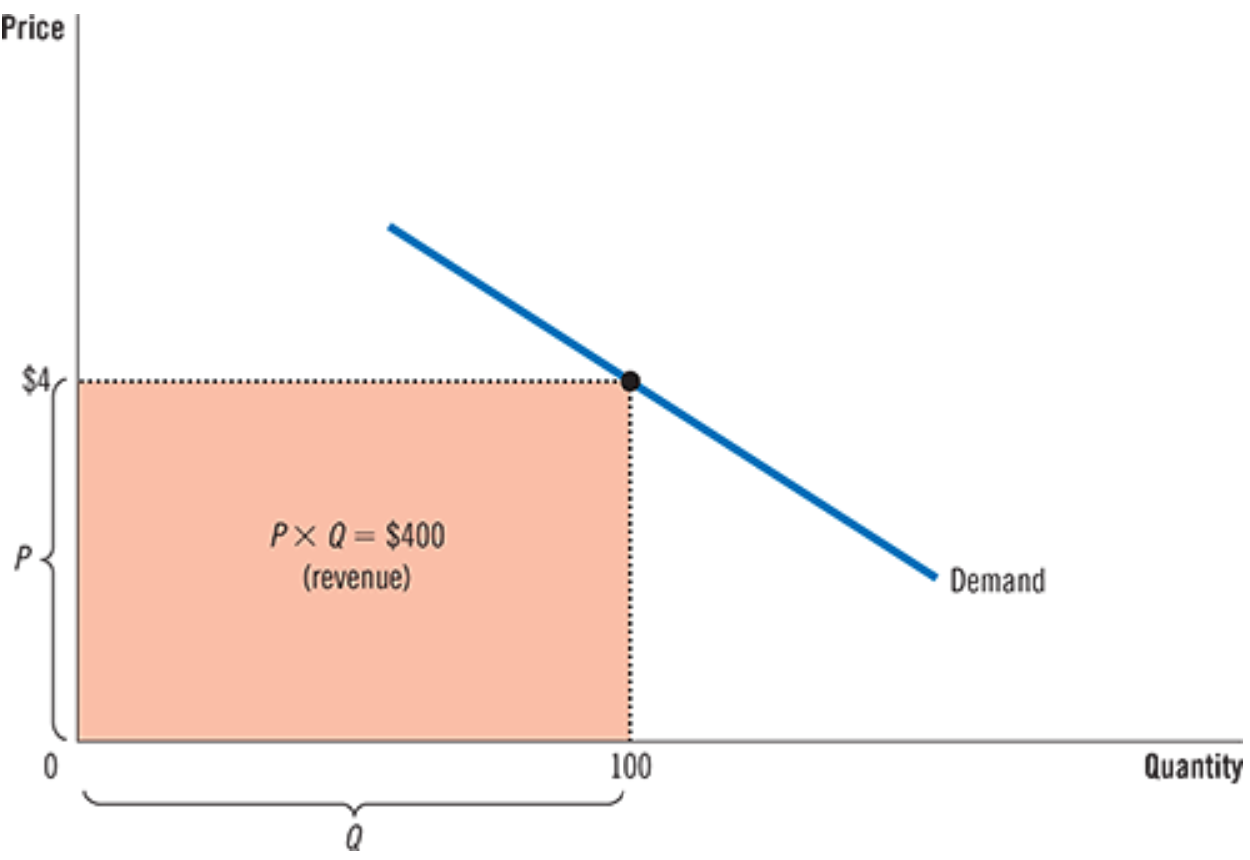
\includegraphics[width=6cm]{total revenue.png}
        \end{figure}
    \end{itemize}
\end{frame}

\begin{frame}{Effects from Raising Prices}
    \begin{itemize}[<+->]
        \item Suppose I raise the price of the good, from \$4 to \$5. Two things happen:
        \begin{itemize}
            \item Price effect: each sale occurs at a higher price than before, raising revenues
            \item Quantity effect: since the price is higher and we are under the law of demand, I will sell less units, lowering revenues
        \end{itemize}
        \item Therefore, whichever of these effects is greater determines whether my TR increases or decreases
        \item Some general rules:
        \begin{itemize}[<2->]
            \item When demand is inelastic (a price elasticity less than one), price and total revenue move in the same direction: If the price increases, total revenue also increases.
            \item When demand is elastic (a price elasticity greater than one), price and total revenue move in opposite directions: If the price increases, total revenue decreases.
            \item If demand is unit elastic (a price elasticity exactly equal to one), total revenue remains constant when the price changes
        \end{itemize}
    \end{itemize}
\end{frame}

\begin{frame}{Effects from Raising Prices, Visually}
        \begin{figure}
            \centering
            \captionsetup{singlelinecheck=off}
            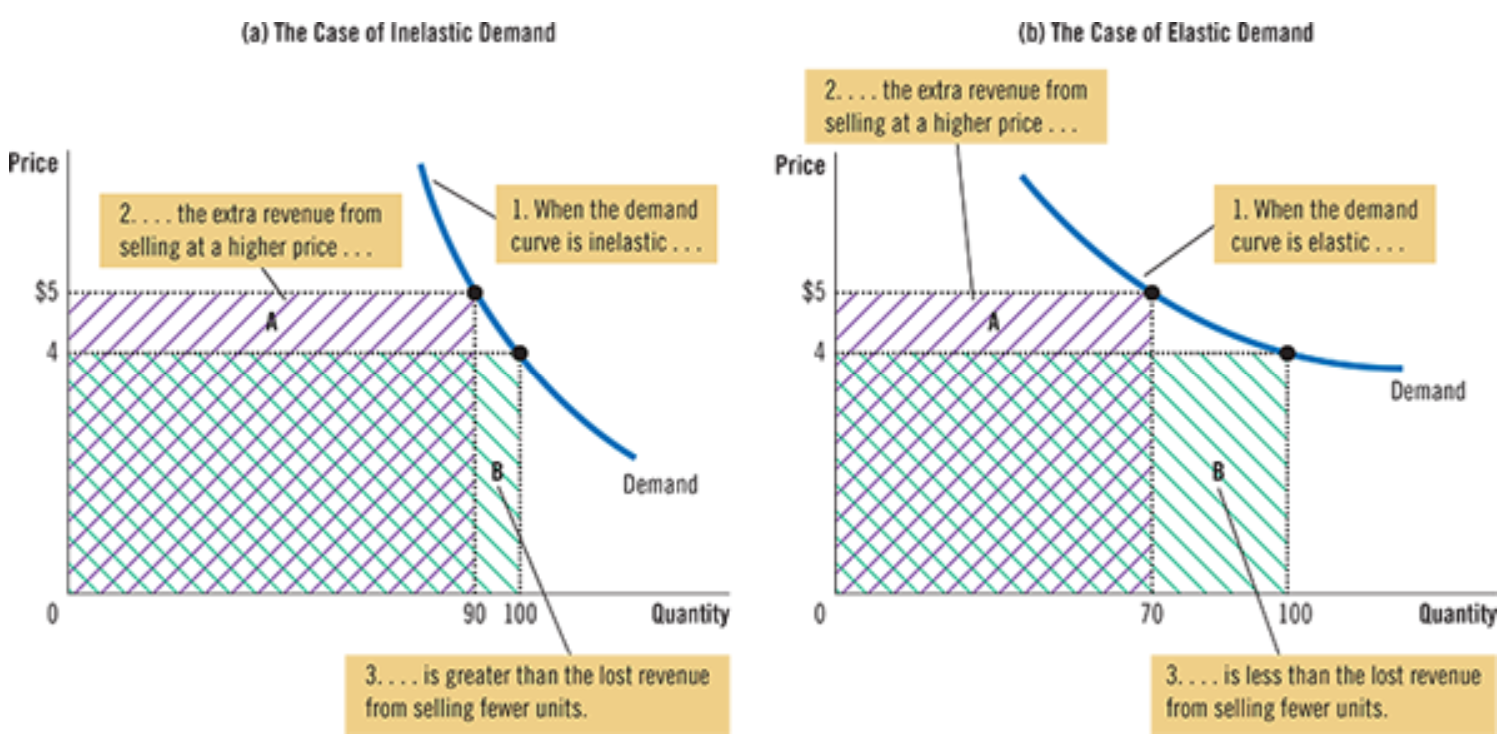
\includegraphics[width=9cm]{ped and tr.png}
            \caption*{\textcolor{pine_green}{\textbullet}\hspace{2mm} ``A" represents the price effect: I am selling goods at a higher price, raising revenue. ``B" represents the quantity effect: I am selling less goods overall, lowering revenue}\pause
            \vspace{-4mm}
            \caption*{{\textcolor{pine_green}{\textbullet}}\hspace{2mm} Change in total revenue ($\Delta TR$) is given by $A-B$. Thus, if $A-B>0$, i.e. if $A>B$, then $\Delta TR>$}
        \end{figure}
\end{frame}

\begin{frame}{Effects from Raising Prices, Visually (cont.)}
        \begin{figure}
            \centering
            \captionsetup{singlelinecheck=off}
            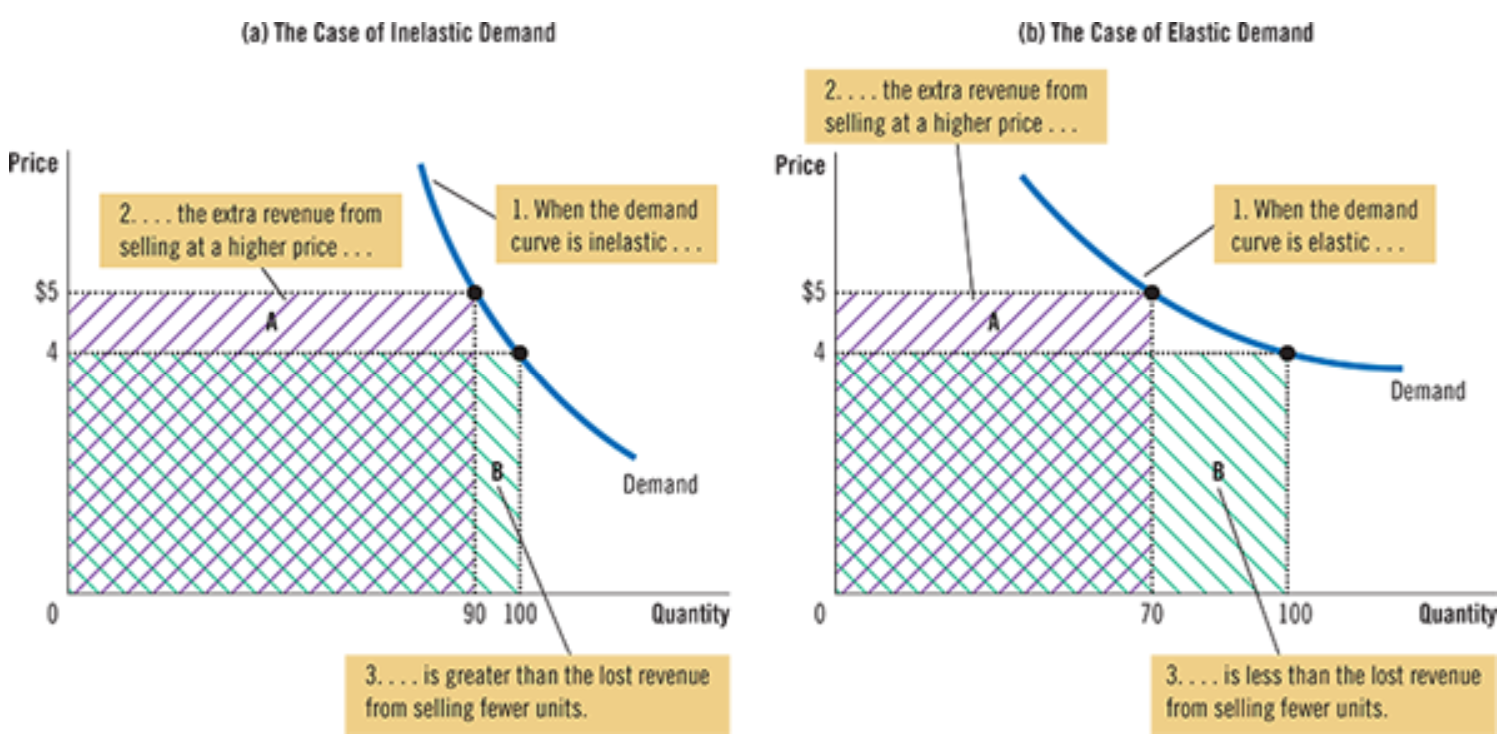
\includegraphics[width=9cm]{ped and tr.png}
            \caption*{\textcolor{pine_green}{\textbullet}\hspace{2mm} In (a), $A=1(90)=90$ and $B=4(10)=40$. In (b), $A=1(70)=70$ and $B=4(30)=120$}\pause
            \vspace{-4mm}
            \caption*{{\textcolor{pine_green}{\textbullet}}\hspace{2mm} When demand is inelastic and people are insensitive to the price, $A>B$, so TR increases. When demand is elastic and people are sensitive to prices, $B>A$, so TR decreases}
        \end{figure}
\end{frame}

\begin{frame}{PED and Total Revenue}
    \begin{itemize}[<+->]
        \item Some general rules:
        \begin{itemize}[<2->]
            \item When demand is inelastic (a price elasticity less than one), price and total revenue move in the same direction: If the price increases, total revenue also increases.
            \item When demand is elastic (a price elasticity greater than one), price and total revenue move in opposite directions: If the price increases, total revenue decreases.
            \item If demand is unit elastic (a price elasticity exactly equal to one), total revenue remains constant when the price changes
        \end{itemize}
        \item Keep in mind that total revenue \underline{is not} the same as profit. This does not factor in the costs to the supplier, it is simply meant to demonstrate a relationship between changes in price and changes in revenues
    \end{itemize}
\end{frame}

\section*{Other Elasticises of Demand}

\begin{frame}{Other Elasticises of Demand}
    \begin{itemize}[<+->]
        \item Recall that the price-elasticity of demand is given by 
        $$\epsilon_{D}=\abs*{\frac{\%\Delta Q_{D}}{\%\Delta P}}$$
        \item This gives the sensitivity of quantity demanded when there is a change in price. But what about the sensitivity in quantity demanded when we change something other than price?
        \item We could certainly put a lot of different things in for change in price, but there are only a few that are common enough to talk about
    \end{itemize}
\end{frame}

\begin{frame}{Income Elasticity of Demand}
    \begin{itemize}[<+->]
        \item The first is the \underline{\textbf{Income Elasticity of Demand}}, which is defined as 
        $$\epsilon_{\i}=\frac{\%\Delta Q_{D}}{\%\Delta \i}$$
        \item Note that $\epsilon_{D}^{\i}$ is common, and has the advantage of clearly communicating that this is a demand elasticity
        \begin{itemize}
            \item I omit the subscript-$D$ here to avoid cluttered notation
            \item Recall that you can replace $\epsilon$ with $e$ or $E$, if you'd like
        \end{itemize}
        \item This measures how sensitive the quantity demanded in a market is when consumers experience a change in \textit{income}    
    \end{itemize}
\end{frame}

\begin{frame}{Interpretation of Income Elasticity of Demand}
    \begin{itemize}[<+->]
        \item $\epsilon_{\i}$ measures how sensitive the quantity demanded in a market is when consumers experience a change in \textit{income}
        \item Note that this is still tied to a \underline{single} good/market at a time
        \item The interpretation of $\epsilon_{\i}$ is similar to PED: when consumers' income rise by by $1\%$, the quantity demanded for good $x$ changes by $\epsilon_{\i}\%$
        \item What sign should the sign of $\epsilon_{\i}$ be? 
        \begin{itemize}
            \item Recall that when income rises, we often expect quantity demanded for a good to rise, in response
            \item So, this number will often be positive
            \item However, we also briefly mentioned in a previous lecture that an increase in income can lead to a drop in $Q_{D}$, \textit{for certain goods}
            \begin{itemize}
                \item These goods are called \textit{inferior}, and they cause $\epsilon_{\i}$ to be negative
                \item Ex: Top ramen, public transit, payday loans, house-brand items, etc.
            \end{itemize}
        \end{itemize}
        \item Since $\epsilon_{D}$ (PED) was always negative, it was fine to throw absolute values on it; since $\epsilon_{\i}$ can be positive or negative, we ought to report it's true sign
    \end{itemize}
\end{frame}

\begin{frame}{Income Elasticity of Demand, by numbers}
    \begin{itemize}[<+->]
        \item A good is said to be \textit{inferior} if $\epsilon_{\i}<0$
        \item A good is said to be \textit{normal} if $0\leq\epsilon_{\i}\leq 1$
        \item A good is said to be a \textit{luxury} (or \textit{superior}) if $\epsilon_{\i}>1$
        \begin{itemize}
            \item This means that $\%\Delta Q_{D}>\%\Delta \i$: the percent change in quantity demanded exceeds the percent change in $\i$
            \item Straightforward examples include yachts, wagyu steak, tailored suits, etc. However, goods such as movies, meals at restaurants, and airline travel can also all be luxury goods
        \end{itemize}
    \end{itemize}
\end{frame}

\begin{frame}{Exercise 2}
    \begin{itemize}[<+->]
        \item Consider the following table for mushrooms
        \begin{figure}
            \centering
            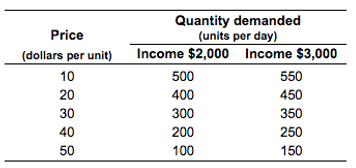
\includegraphics[width=7cm]{income elasticity example.jpg}
        \end{figure}
        \item Find the income elasticity [of demand] when  $p=\$30$. Are mushrooms inferior, normal, or superior?
    \end{itemize}
\end{frame}

\begin{frame}{Solution 2}
    \begin{itemize}[<+->]
        \item The income elasticity when $p=\$30$ is given by 
        \begin{align*}
            \epsilon_{\i}&=\frac{(350-300)/[(350+300)/2]}{(3000-2000)/[(2000+3000)/2]}\\
            &=\frac{50/325}{1000/2500}\\
            &=\frac{2/13}{2/5}\\
            &=\frac{5}{13}\approx0.39
        \end{align*}
        \item When consumers' income rises by 1\%, we expect the quantity demanded for mushrooms to rise by 0.39\%
        \item Thus, the mushrooms are normal
        \item Note: I didn't specify whether income went up or down. In this case, it does not matter which direction you chose, as long as you were consistent (I did $2000\to 3000$, so $300\to350$; $3000\to 2000$ would mean $350\to300$)
    \end{itemize}
\end{frame}

\begin{frame}{Cross-Price Elasticity of Demand}
    \begin{itemize}[<+->]
        \item The other demand elasticity we will talk about is the \underline{\textbf{Cross-Price}} \underline{\textbf{Elasticity of Demand}} (CPED)\footnote{\vspace{1mm} As an aside, the existence of cross-price elasticity of demand leads some economists to refer to the price elasticity of demand as the ``\textit{Own} price elasticity of demand"}
        \item For this elasticity, we need two goods: $X$ and $Y$
        \item Important: The Cross-Price Elasticity of Demand \textit{for good $x$ with respect to good $x$} is defined as 
        $$\epsilon_{xy}=\frac{\%\Delta Q_{x}}{\%\Delta P_{y}}$$
        \item The important part here is the order, as it is easy to get confused which good goes on the top versus which one goes on the bottom
        \item Here, $Q_{x}$ is still taken to be the quantity demanded ($Q_{D}$) of $x$, but I have omitted $D$ to avoid clutter\footnote{\vspace{1mm}You can write $Q_{D_{x}}$, if you would like}
    \end{itemize}
\end{frame}

\begin{frame}{Interpretation of CPED}
    \begin{itemize}[<+->]
        \item The textbook defines CPED as the ``measure of how much the quantity demanded of one good responds to a change in the price of another good, computed as the percentage change in quantity demanded of the first good divided by the percentage change in price of the second good"
        \item In a similar style to the other elasticities, if the cross price elasticity of $x$ with respect to $y$ is given by $\epsilon_{xy}$, then we say that if the price of $y$ rises by 1\%, then the quantity demanded for good $x$ changes by $\epsilon_{xy}\%$ 
    \end{itemize}
\end{frame}

\begin{frame}{Purpose of CPED}
    \begin{itemize}[<+->]
        \item The reason we use CPED is to determine whether two goods are complements or substitutes -- let's think about which sign should be which
        \item When $y$ is a substitute for $x$, we expect that an increase in the price of $y$ leads to a(n)...
        \begin{itemize}
            \item increase in the quantity demanded of $x$, meaning $\epsilon_{xy}$ should be...
            \item positive
        \end{itemize}
        \item Likewise, when $y$ is a complement to $x$, we expect that an increase in the price of $y$ leads to a decrease in the quantity demanded of $x$, so $\epsilon_{xy}$ should be negative
    \end{itemize}
\end{frame}

\begin{frame}{CPED, by numbers}
Goods $x$ and $y$ are said to be...
    \begin{itemize}[<+->]
        \item \textit{complements} if $\epsilon_{xy}<0$
        \begin{itemize}
            \item \textit{perfect complements} if $\epsilon_{xy}=-\infty$
            \begin{itemize}
                \item Close example: left and right shoes
            \end{itemize}
        \end{itemize}
        \item \textit{unrelated} if $\epsilon_{xy}=0$
        \item \textit{substitutes} if $\epsilon_{xy}<0$
        \begin{itemize}
            \item \textit{perfect substitutes} if $\epsilon_{xy}=\infty$
            \begin{itemize}
                \item Close example: any goods which are similar enough for you to only care about price: two brands of butter, triple sec, cheap coffee, etc.
            \end{itemize}
        \end{itemize}
    \end{itemize}
\end{frame}

\begin{frame}{An Obscure Aside}
    \begin{itemize}[<+->]
        \item Q: Is the CPED symmetric? I.e., does $\epsilon_{xy}=\epsilon_{yx}$?
        \begin{itemize}
            \item An increase in the price of a gaming console means less video games will get consumed, but does that mean that if video games get more expensive, people will reduce their console consumption by a similar amount?
            \item Alternatively, do you think that a change in the price of sprite will affect the demand for coke in the exact same way that a change in the price of coke will affect the demand for sprite? 
        \end{itemize}
        \item A: Probably not, so an interesting fact of CPEDs is that they are not necessarily symmetric
        \item Any interesting examples you can think of?
    \end{itemize}
\end{frame}

\begin{frame}{Exercise 3}
    \begin{itemize}[<+->]
        \item Suppose that when berries rise in price by 16\%, the demand for cream falls from 20 oz to 18 oz
        \item However, when the price of cream rises by 16\%, the demand for berries falls from 30 oz to 20 oz
        \item Calculate $\epsilon_{bc}$ and $\epsilon_{cb}$. Are berries and cream substitutes, complements, or neither?
    \end{itemize}
\end{frame}

\begin{frame}{Solution 3}
    \begin{itemize}[<+->]
        \item \begin{align*}
            \epsilon_{bc}=\frac{[(20-18)/19]\cdot 100}{16}=\frac{10.53}{16}=0.658
        \end{align*}
        \item \begin{align*}
            \epsilon_{cb}=\frac{[(30-20)/25]\cdot 100}{16}=\frac{40}{16}=2.5
        \end{align*}
        \item The goods are complements, note that they are asymmetric
    \end{itemize}
\end{frame}

\begin{frame}{Elasticity and Ceteris Paribus}
    \begin{itemize}[<+->]
        \item Recall my ceteris paribus example:
        \begin{itemize}
            \item You want to find the impact that time of year has on gas prices, so you decide to compare gas price averages across different months: Jan-Jan, Feb-Feb, etc. Your sample years are 2020 and 2021
        \end{itemize}
        \item Picking 2020 and 2021 will not give you an accurate measure of how time of year impacts gas, because COVID had such large impacts on everything
        \item In the same spirit, what would happen if the price of good $x$ changed between the two data points you were using to calculate income elasticity?
    \end{itemize}
\end{frame}

\begin{frame}{Elasticity and Ceteris Paribus (cont.)}
    \begin{figure}
        \centering
        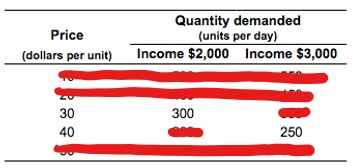
\includegraphics[width=7cm]{cet_par example 1.jpg}
        \caption*{I have two points with different $Q_{D}$ and $\i$. Can you calculate income elasticity using these two data points? What about PED?}
    \end{figure}
\end{frame}

\begin{frame}{Elasticity and Ceteris Paribus (cont.)}
    \begin{itemize}[<+->]
        \item Suppose you land a job at Amazon, and are tasked with calculating the price elasticity of demand for soda
        \item After a year of market research, you find the price elasticity of demand for Dr. Pepper 0.82
        \item However, you neglected to notice that Pibb Xtra (Mr. Pibb) was running huge sales all year. Is that a big deal?
        \item A: \textbf{yes}. There are problems with all of these. Without keeping everything else constant, we have no way to separate out the effects from different price and income movements
        \begin{itemize}
            \item You can't know that a 1\% increase in price decreases demand for Dr. Pepper by 0.82\%, because, for all you know, most of the demand decrease you saw came from Mr. Pibb sales
            \item Likewise, the decrease in the demand for mushrooms could very well have been from the price increase (we actually know it is, because we found mushrooms to be a normal good earlier). Moreover, the income change increase could have stunted this observation about price elasticity
        \end{itemize}
    \end{itemize}
\end{frame}

\begin{frame}{Takeaway}
    \begin{itemize}[<+->]
        \item To effectively calculate elasticities, you have to have other relevant factors held constant
        \item This is the tough task of many experimental and data-driven economists: finding data and using techniques such that you can isolate meaningful results that you are confident in
    \end{itemize}
\end{frame}

\begin{frame}{Comments}
    \begin{itemize}
        \item I will cover 5-2 on Monday
        \item Read 5-3 on your own
        \item You can start the homework, but you may want to wait until after Monday before you get too far
    \end{itemize}
\end{frame}





\end{document}